\documentclass[11pt, wide, leqno]{mwart}

\usepackage{../template}

\tit{P.0.12.}

\begin{document}
\maketitle
\tableofcontents

\section{Wstęp}\label{sec:ws}

W matematyce bardzo często pojawiają się wartości niewymierne, takie jak $\ln \frac12$, których nie możemy wyrazić w sposób przystępny dla człowieka. Z tego powodu, powstało wiele metod przybliżania funkcji w określonych punktach. Jedną z nich jest użycie szeregu Taylora, opisanego przez Brooka Taylora w 1715 roku oraz wspomniana przez Jamesa Gregory'a w 1671 r.

W swojej istocie twierdzenie Taylora mówi, że jeśli dana jest funkcja $f$ klasy $C^n$, czyli różniczkowalna $n$ razy w każdym punkcie jej dziedziny, to możemy ją przybliżyć w otoczeniu dowolnego punktu $a$ za pomocą szeregu:
$$f(x)=\sum\limits_{k=0}^n\big({(x-a)^k\over k!} f^{(k)}(a)\big)+R_n(x, a),$$
gdzie $R_n(x, a)$ spełnia
$$\lim\limits_{x\to a}{R_n(x,a)\over\|x-a\|^n}=0.$$
Jak nietrudno zauważyć, wartość $R_n(x, a)$ przy $x$ bardzo blisko $a$ jest zaniedbywalnie mała, więc w trakcie obliczeń możemy ją pominąć.

Celem niniejszego sprawozdania jest sprawdzenie dokładności przybliżania funkcji za pomocą szeregów Taylora. W \$\$ omówione zostanie przybliżanie ustalonych wartości funkcji $\ln x$ w punkcie $x=\frac12$. Wykorzystany zostanie szereg Maclaurina funkcji $\ln(x+1)$ w okolicach $x=0$ dla stopni wielomianu $n=1, 2, ..., 16$. Wyniki porównane zostaną z wynikiem bibliotecznej funkcji \verb+log(x)+ w języku Julia. Otrzymane dane zostaną zaprezentowane w formie tabeli oraz grafów otrzymanych za pomocą załączonego w pliku \verb+program.jl+. Dodatkowo, funkcje użyte w programie zostaną zaprezentowane w formie Jupyter Notebook w pliku \verb+program.ipynb+.

\section{Przybliżanie wartości $\ln\frac12$}

\subsection{Metoda}

W celu obliczenia wartości $\ln\frac12$ użyte zostanie przybliżanie funkcji
$$f(x)=\ln (1+x)$$
w pobliżu $a=0$ za pomocą szerega Maclaurina.

Wzór na pochodną funkcji $\ln (x+1)$ jest powszechnie znany:
$${d\over dx}\ln (x+1)=\frac1{x+1},$$
natomiast wzór na pochodną $k$-tego stopnia, można wyliczyć w prosty sposób:
\begin{align}
    {d^k\over dx^k}\ln (x+1)=(-1)^{k+1}{(k-1)!\over(1+x)^{k}}.
\end{align}

Wzór na szereg Taylora $\ln (1+x)$ w pobliżu $a=0$, to:
$$f(0)=\sum\limits_{i=0}^n{f^{(k)}(x)\over k!}(x-0)^n + R(x, 0)=\sum\limits_{i=1}^n(-1)^{i+1}{x^i\over i}+R(x, 0).$$

\subsection*{Wyniki}

Wyniki oszacowań wartości $\ln\frac12$ zostały zaprezentowane na ~Grafie~\ref{fg:val}, natomiast wartości błędów są widoczne w~Tabeli~\ref{tab:ksks} oraz na~Grafie~\ref{fg:err}.

\begin{table}[h!]
    \centering
    \begin{tabular}{| c | c | c |}
        \hline
        Stopień wielomianu & Błąd bezwzględny & Błąd względny\\
        \hline
        1 & 0.193147 & 0.278652\\
        \hline
        2 & 0.0681472   &    0.0983156 \\
        \hline
        3 & 0.0264805   &    0.0382033 \\
        \hline
        4 & 0.0108555    &   0.0156612 \\
        \hline
        5 & 0.00460551   &   0.00664435 \\
        \hline
        6 & 0.00200135   &   0.00288733 \\
        \hline
        7 & 0.000885276  &   0.00127718 \\
        \hline
        8 & 0.000396995  &   0.000572742 \\
        \hline
        9 & 0.000179981 & 0.000259657 \\
        \hline
        10 & 8.23244e-5 & 0.000118769 \\
        \hline
        11 & 3.79352e-5   &   5.47289e-5 \\ 
        \hline
        12 & 1.75902e-5  &    2.53772e-5 \\
        \hline
        13 & 8.20013e-6   &   1.18303e-5 \\
        \hline
        14 & 3.84047e-6   &   5.54063e-6 \\
        \hline
        15 & 1.80597e-6   &   2.60546e-6 \\
        \hline
        16 & 8.52295e-7  &    1.2296e-6 \\
        \hline
    \end{tabular}
    \caption{Błąd bezwzględny i względny otrzymanego wyniku w stosunku do funkcji bibliotecznej w zależności od stopnia wielomianu użytego do obliczeń.\label{tab:ksks}}
\end{table}

\begin{figure}[h!]
    \centering
    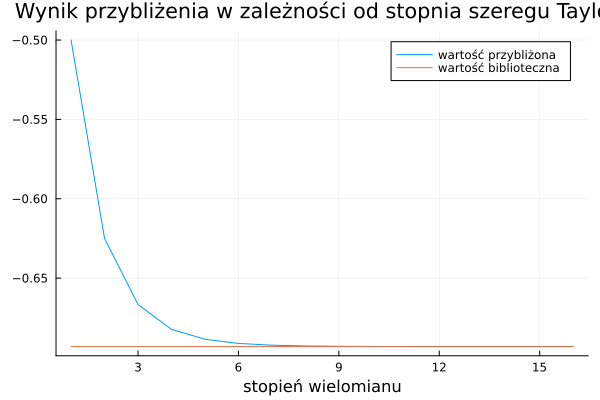
\includegraphics[scale=0.6]{./prog/val_plot.png}
    \caption{Wyniki programu dla różnych stopni wielomianu z naniesioną wartością funkcji bibliotecznej.\label{fg:val}}
\end{figure}

\begin{figure}[h!]
    \centering
    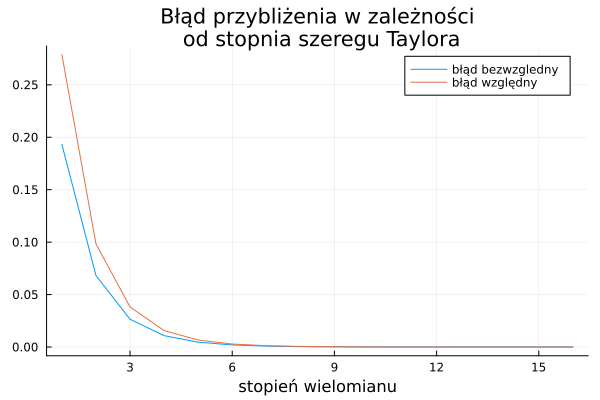
\includegraphics[scale=0.6]{./prog/err_plot.png}
    \caption{Zależność między wartością bezwzględną błędów względnego i bezwzględnego a stopniem wielomianu.\label{fg:err}}
\end{figure}

\newpage

~Graf~\ref{fg:err} pokazuje, że wraz ze wzrostem stopnia wielomianu używanego do przybliżenia poszukiwanej wartośći dokladność rośnie niemalże wykładniczo. Dla wielomianów stopnia co najmniej 9 oba błędy stają się bliskie zero tak, że możemy je pomijać dla obliczeń na \verb+Float64+. Możliwe też jest, że funkcja biblioteczna opiera się na metodzie analogicznej do zaprezentowanej w powyższej pracy.

\koniec
\end{document}